% Options for packages loaded elsewhere
\PassOptionsToPackage{unicode}{hyperref}
\PassOptionsToPackage{hyphens}{url}
%
\documentclass[
]{book}
\usepackage{lmodern}
\usepackage{amssymb,amsmath}
\usepackage{ifxetex,ifluatex}
\ifnum 0\ifxetex 1\fi\ifluatex 1\fi=0 % if pdftex
  \usepackage[T1]{fontenc}
  \usepackage[utf8]{inputenc}
  \usepackage{textcomp} % provide euro and other symbols
\else % if luatex or xetex
  \usepackage{unicode-math}
  \defaultfontfeatures{Scale=MatchLowercase}
  \defaultfontfeatures[\rmfamily]{Ligatures=TeX,Scale=1}
\fi
% Use upquote if available, for straight quotes in verbatim environments
\IfFileExists{upquote.sty}{\usepackage{upquote}}{}
\IfFileExists{microtype.sty}{% use microtype if available
  \usepackage[]{microtype}
  \UseMicrotypeSet[protrusion]{basicmath} % disable protrusion for tt fonts
}{}
\makeatletter
\@ifundefined{KOMAClassName}{% if non-KOMA class
  \IfFileExists{parskip.sty}{%
    \usepackage{parskip}
  }{% else
    \setlength{\parindent}{0pt}
    \setlength{\parskip}{6pt plus 2pt minus 1pt}}
}{% if KOMA class
  \KOMAoptions{parskip=half}}
\makeatother
\usepackage{xcolor}
\IfFileExists{xurl.sty}{\usepackage{xurl}}{} % add URL line breaks if available
\IfFileExists{bookmark.sty}{\usepackage{bookmark}}{\usepackage{hyperref}}
\hypersetup{
  pdftitle={Standard Operating Procedures for Advanced UAS Operations},
  hidelinks,
  pdfcreator={LaTeX via pandoc}}
\urlstyle{same} % disable monospaced font for URLs
\usepackage{longtable,booktabs}
% Correct order of tables after \paragraph or \subparagraph
\usepackage{etoolbox}
\makeatletter
\patchcmd\longtable{\par}{\if@noskipsec\mbox{}\fi\par}{}{}
\makeatother
% Allow footnotes in longtable head/foot
\IfFileExists{footnotehyper.sty}{\usepackage{footnotehyper}}{\usepackage{footnote}}
\makesavenoteenv{longtable}
\usepackage{graphicx,grffile}
\makeatletter
\def\maxwidth{\ifdim\Gin@nat@width>\linewidth\linewidth\else\Gin@nat@width\fi}
\def\maxheight{\ifdim\Gin@nat@height>\textheight\textheight\else\Gin@nat@height\fi}
\makeatother
% Scale images if necessary, so that they will not overflow the page
% margins by default, and it is still possible to overwrite the defaults
% using explicit options in \includegraphics[width, height, ...]{}
\setkeys{Gin}{width=\maxwidth,height=\maxheight,keepaspectratio}
% Set default figure placement to htbp
\makeatletter
\def\fps@figure{htbp}
\makeatother
\setlength{\emergencystretch}{3em} % prevent overfull lines
\providecommand{\tightlist}{%
  \setlength{\itemsep}{0pt}\setlength{\parskip}{0pt}}
\setcounter{secnumdepth}{5}
\usepackage{booktabs}
\usepackage{amsmath}
\usepackage{amsfonts}
\usepackage{amssymb}
\usepackage{graphicx}
\usepackage[left=2cm,right=2cm,top=2cm,bottom=2cm]{geometry}
\usepackage[]{natbib}
\bibliographystyle{apalike}

\title{Standard Operating Procedures for Advanced UAS Operations}
\author{}
\date{\vspace{-2.5em}}

\begin{document}
\maketitle

{
\setcounter{tocdepth}{1}
\tableofcontents
}
\hypertarget{ch-getting-started}{%
\chapter{Drone Guide Portal}\label{ch-getting-started}}

\begin{center}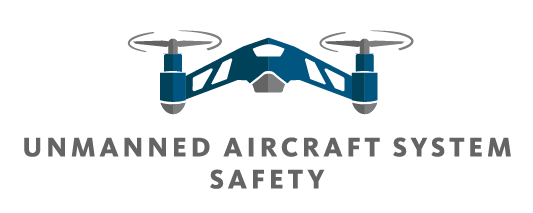
\includegraphics[width=0.5\linewidth]{images/COE_logo} \end{center}

This is Standard Operating Procedures for Advanced UAS Operations. This manual is intended to promote safe and efficient UAS operations by any operator operating a UC-owned UAS or operating a personally owned UAS for University Business for non-standard UAS activity. This includes the use of UAS in moderate and above Risk Levels, the use of UAS in conjunction with a UC Airspace Waiver or Operational Waiver.

Further information regarding the operation of UAS may be found within the Presidential Unmanned Aircraft System Policy and/or the \href{https://ucdrones.github.io/Policy_Guidance/}{UAS Policy Guidance Document}.

This page will be a work in progress and new resources will be added periodically. Feel free to reach out to us at \href{mailto:UASSafety@ucmerced.edu}{\nolinkurl{UASSafety@ucmerced.edu}} if you have any questions or would like to see additional resources added.

\hypertarget{ch-scope}{%
\chapter{Scope}\label{ch-scope}}

The Standard Operating Procedures for Advanced UAS Operations (SOPA) has been prepared for the use and guidance of UAS in flight operations, flight planning, training, and oversight as a requirement to exercise the privileges of operating under 1) a Grant of Exemption pursuant to Section 333 of the FAA Modernization and Reform Act of 2012, 2) any Public Agency Operation when operating a Public Aircraft, 3) any other operations conducted under a Certificate of Waiver or Authorization (COA) including an Airspace Authorization, Airspace Waiver or Operational Waiver or 4) any operation categorized as a moderate and above Risk Level.

\begin{quote}
The SOPA does not address every possible contingency that may arise or every rule of safety and good practice. In addition to the SOPA, operators of UAS are expected to be aware of their surroundings and take into account any special characteristics of the area or the mission being flown.
\end{quote}

All faculty, staff, students, and other personnel operating under the privileges of the UC's Grant of Exemption, and any COAs, must be in compliance with all applicable Federal Aviation Regulations, and State and local laws. To the extent of any inconsistencies between the minimum requirements set in the UC UAS Policy, the Policy Guidance Document, or the SOPA and any applicable regulation, the regulatory requirements govern.

\begin{quote}
The SOPA must be read in conjunction with the UC's Grant of Exemption and any applicable COA issued to the UC by the FAA. Copies of these documents should be included as an Appendix to the SOPA before conducting UAS activity. The SOPA, including any revised documents, must be made available to the FAA upon request. To download a copy of this SOPA, click the download options (PDF, ePUB) in the header bar.
\end{quote}

The SOPA is intended to be a convenient source of the UC's advanced or non-standard UAS operation procedures. Everyone participating in applicable UAS activity should study this entire Manual to familiarize themselves with its requirements before participating in any UAS activity for University business.

Always remember -- everyone operating a UAS under the University's banner shares responsibility for compliance and ensuring safety.
Good luck and fly safely!

\hypertarget{ch-roles-responsibilities}{%
\chapter{Roles and Responsibilities}\label{ch-roles-responsibilities}}

\hypertarget{systemwide-designated-uas-authority}{%
\section{Systemwide Designated UAS Authority}\label{systemwide-designated-uas-authority}}

The Systemwide Designated UAS Authority provides expertise, support and training for regulatory compliance, risk management and the safe operation of UAS across the UC system. Further information regarding the roles and responsibilities of the Systemwide Designated UAS Authority can be found within the UC UAS Policy and the \href{https://ucdrones.github.io/Policy_Guidance/}{UAS Policy Guidance Document}.

\hypertarget{duties-and-responsibilities}{%
\subsection{Duties and Responsibilities}\label{duties-and-responsibilities}}

\begin{itemize}
\tightlist
\item
  Ensure that UC faculty, staff, and students participating in University UAS activity are aware of their compliance responsibilities under the Federal Regulations, State and Local Laws, any applicable COAs, and this SOPA.
\item
  Maintain a current master copy of this SOPA.
\item
  Serve as the primary point of contact with the FAA.
\item
  Promote compliance with FAA or NTSB reporting requirements.
\item
  Coordinate and promote compliance with applicable record-keeping requirements as specified under this SOPA.
\item
  The Systemwide Designated UAS Authority may delegate functions to other personnel, including Designated Local Authorities for UAS activity at the campus/locations where activities are conducted.
\end{itemize}

\hypertarget{designated-local-authority}{%
\section{Designated Local Authority}\label{designated-local-authority}}

The Designated Local Authority is a single-point of contact or committee appointed by the Chancellor, Vice Chancellors, or Deans at an individual University Location to oversee the development, implementation, and enforcement of any University Location-specific UAS related policies and procedures. Further information regarding the roles and responsibilities of the Designated Local Authority can be found within the UC UAS Policy and the \href{https://ucdrones.github.io/Policy_Guidance/}{UAS Policy Guidance Document}.

\hypertarget{duties-and-responsibilities-1}{%
\subsection{Duties and Responsibilities}\label{duties-and-responsibilities-1}}

\begin{itemize}
\tightlist
\item
  Is responsible for regulatory compliance and risk management of UAS activity within their authority.
\item
  Maintains a list of UAS UAS activity.
\item
  Coordinates UAS activity across multiple departments for appropriate reviews.
\item
  Ensures UAS liability insurance coverage for all activity.
\item
  Reviews and interprets applicable regulations and policies at the campus-level.
\item
  Serve as the liaison between regulatory agencies and the operators.
\end{itemize}

\hypertarget{remote-pilot-in-command}{%
\section{Remote Pilot in Command}\label{remote-pilot-in-command}}

The RPIC of the UAS shall be the person who as the final authority and responsibility for the operation and safety of an sUAS operation as described by 14 CFR 107.19 for sUAS or 14 CFR 91.3 for UAS when operating as Public Aircraft or under the Section 333 Grant of Exemption.

The RPIC has ultimate responsibility for the safe operation of the UAS. As a result, the RPIC has the final decision on whether to initiate or terminate any flight.

\hypertarget{duties-and-responsibilities-2}{%
\subsection{Duties and Responsibilities}\label{duties-and-responsibilities-2}}

\begin{itemize}
\tightlist
\item
  The RPIC will evaluate each UAS activity in detail prior to operation. It is the responsibility of the RPIC to recognize and refuse any UAS activity that in the RPIC's judgment is not safe. The RPIC's word is final as to whether the UAS activity is feasible and can be conducted in a safe and efficient manner.
\item
  The RPIC must understand the UAS activity and have all applicable maps, charts and manuals available while on-site. Additionally, the RPIC is required to be aware of weather forecasts, winds, hazards, temporary flight restrictions, and all pertinent information necessary to perform the UAS activity.
\item
  The RPIC is responsible for ensuring that all documentation has been completed, submitted and accepted, including submission of the UAS Activity Request Form, filing of any necessary notices, and any necessary flight plans or safety mitigation analysis.
\end{itemize}

\hypertarget{qualifications}{%
\subsection{Qualifications}\label{qualifications}}

\begin{itemize}
\tightlist
\item
  It is the responsibility of the RPIC to ensure that he or she has current and sufficient experience with the UAS to be utilized in the non-standard UAS operation.
\item
  The RPIC must have a remote pilot certificate with a small UAS rating issued pursuant to subpart C of 14 CFR Part 107, or any other certificate or license required for the operation being conducted.
\item
  The RPIC must maintain an understanding of the normal, abnormal and emergency procedures of the UAS.
\item
  The RPIC must maintain an appropriate level of understanding of the operating flight rules in the airspace where the UAS operations will occur.
\end{itemize}

\hypertarget{visual-observer}{%
\section{Visual Observer}\label{visual-observer}}

A Visual Observer is a person designated by the RPIC to assist the RPIC and the person manipulating the flight controls of the UAS to see and avoid other air traffic or objects aloft or on the ground.

\hypertarget{duties-and-responsibilities-3}{%
\subsection{Duties and Responsibilities}\label{duties-and-responsibilities-3}}

\begin{itemize}
\tightlist
\item
  A Visual Observer is responsible for assisting the RPIC in maintaining situational awareness and complying with `see-and-avoid' by scanning the area around the UAS for potentially conflicting traffic or other hazards to the safety of the flight.
\item
  A Visual Observer will maintain verbal contact with the RPIC at all times and be able to advise the RPIC of any hazards that arise during flight. Intermittent forms of communications (texting, email, messaging systems) are not acceptable means of compliance. A cell-phone is acceptable if the connection was made prior to launch and is connected through the duration of the flight.
\item
  A Visual Observer shall maintain visual contact with the aircraft and maintain visual lookout for any airborne or ground-based threats in accordance with 14 CFR 107.31 or other FAA requirement.
\end{itemize}

\hypertarget{qualifications-1}{%
\subsection{Qualifications}\label{qualifications-1}}

\begin{itemize}
\tightlist
\item
  The Visual Observer must maintain an appropriate level of understanding of the operating flight rules in the airspace where the UAS operations will occur.
\item
  The Visual Observer must maintain an understanding of the normal, abnormal and emergency procedures of the UAS.
\end{itemize}

\hypertarget{ground-support-personnel}{%
\section{Ground Support Personnel}\label{ground-support-personnel}}

A Ground Support Personnel is any person with an assigned responsibility to ensure the safety of the UAS activity but not tasked as the RPIC, Visual Observer, or Payload Operator.

\hypertarget{duties-and-responsibilities-4}{%
\subsection{Duties and Responsibilities}\label{duties-and-responsibilities-4}}

\begin{itemize}
\tightlist
\item
  A Ground Support Personnel is responsible for assisting the RPIC in maintaining situational awareness, providing ground support and other activity to ensure the safety of the flight.
\item
  A Ground Support Personnel may be tasked with supporting launch and recovery operations
\item
  A Ground Support Personnel may be tasked with preventing non-participants from entering the flight area
\item
  A Ground Support Personnel may be tasked with interacting with curious bystanders or spectators
\end{itemize}

\hypertarget{point-of-contact-or-operation-manager}{%
\section{Point of Contact or Operation Manager}\label{point-of-contact-or-operation-manager}}

The Point of Contact or Operation Manager is responsible for the oversight of the UAS activity. The Point of Contact must be documented for all UAS activity. The Point of Contact may also be the RPIC.

\hypertarget{payload-operator-optional}{%
\section{Payload Operator (optional)}\label{payload-operator-optional}}

During UAS activity that might require more complex aerial work, and when the sensor (e.g., camera systems, gimbal) requires the use of a dedicated personnel, the RPIC will be assisted by a Payload Operator. The Payload Operator will be responsible for remotely controlling the movements of camera systems on-board the UAS.

The Payload Operator does not have the authority to require the RPIC to maneuver the aircraft in any unsafe manner or in any manner that violates Federal Regulations.

No one may act as a Payload Operator unless they have read and familiarized themselves with the contents of this SOPA, as well as any additional manuals for the specific payload to be operated.

\hypertarget{ch-UAS}{%
\chapter{Unmanned Aircraft Systems}\label{ch-UAS}}

\begin{itemize}
\item
  Unless otherwise specified, there are no make and model restrictions for the operations of UAS
\item
  All UAS must be operated and maintained in accordance with the recent revision of the UAS Manufacturer's Manual.
\item
  The term `Manufacturer's Manual' as used in this Manual includes all manuals and publications provided by the relevant UAS manufacturer including, but not limited to:

  \begin{itemize}
  \tightlist
  \item
    User Manuals
  \item
    Instruction Manuals
  \item
    Training Manuals
  \item
    Operations Manuals
  \item
    Pilot Operating Handbooks
  \item
    Component Maintenance Manuals
  \item
    Service or Safety Bulletins
  \item
    Service Information Letters
  \end{itemize}
\end{itemize}

\hypertarget{registration-of-uas}{%
\section{Registration of UAS}\label{registration-of-uas}}

Within the US, all UA must be registered under the regulations specified by 14 CFR 47 or 14 CFR 48, depending on the weight of the aircraft, location of the aircraft's operation or primary purpose of the aircraft. Aircraft flown exclusively outside the US or within military airspace may be subject to other registration requirements. In addition, before conducting operations, the radio frequency spectrum used for operation and control of the UAS must comply with the FCC or other appropriate government oversight agency requirements.

\hypertarget{registration-of-uc-owned-uas}{%
\subsection{Registration of UC-owned UAS}\label{registration-of-uc-owned-uas}}

The Regents are the legal owners of all UC property. Similarly to BFB-BUS-19: Registration and Licensing of University-Owned Vehicles, all UC-owned UA must be registered to the ``Regents of the University of California'' to meet compliance obligations under 14 CFR 47 or 14 CFR 48 (See Figure \ref{fig:reg-cert})

\begin{figure}

{\centering 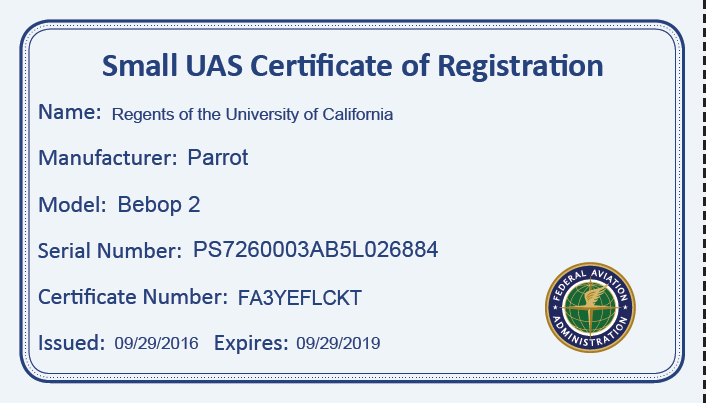
\includegraphics[width=0.5\linewidth]{images/reg_cert} 

}

\caption{Example UAS Registration Certificate}\label{fig:reg-cert}
\end{figure}

All UAS that weigh between 0.55 lbs and 55 lbs (under 14 CFR 48) must be registered online at \url{https://faadronezone.faa.gov/}.

UAS that weigh more than 55 lbs or are required to have UAS registration that is valid internationally must be registered under 14 CFR 47 and must be done through mail with an Original Aircraft Registration Form, AC Form 8050-1.

\begin{quote}
This SOPA does not cover the use of UAS under the Limited Exception for Recreational Use.
\end{quote}

\hypertarget{record-keeping-policy-requirements}{%
\section{Record Keeping Policy Requirements}\label{record-keeping-policy-requirements}}

Records of UC-owned UAS registration must be provided to the Designated Local Authority or the Systemwide Designated UAS Authority. Registration of all unmanned aircraft used for University Business must be provided to the Designated Local Authority or the Systemwide Designated UAS Authority. UC Drones may be used to submit records electronically and other electronic submission processes may be available in the future. A University Location may additionally implement a centralized registration process using a single FAA online account.

\hypertarget{ch-mission-binder}{%
\chapter{UAS Mission Binder}\label{ch-mission-binder}}

The following documentation must be available on-site either electronically or physically upon request, as applicable.

\begin{itemize}
\tightlist
\item
  Remote Pilot Certificate
\item
  sUAS Registration (Either Part 47 Paper or Part 48 Online)
\item
  A copy of any applicable Airspace Authorization, Airspace Waiver or LAANC authorization code
\item
  UC Flight Approval from the Systemwide Designated UAS Authority, Designated Local Authority or other authorized personnel
\item
  A copy of a completed Risk Assessment (may be documented in UC Drones)
\item
  A copy of the Emergency Procedure Checklist for the flight mission - \href{https://ucdrones.github.io/ch-resources.html}{Template Available}
\item
  An up-to-date weather report
\item
  A copy of this Standard Operating Procedures for Advanced Operations (Online, or for off-line access use the download links at the top of the page: pdf or epub available)
\item
  A copy of any applicable COA
\end{itemize}

\hypertarget{ch-flight-planning}{%
\chapter{Flight Planning Procedures}\label{ch-flight-planning}}

The following section outlines the Flight Planning Procedures for UAS activity operating under 1) Grant of Exemption pursuant to Section 333 of the FAA Modernization and Reform Act of 2012, 2) any Public Agency Operation when operating a Public Aircraft, 3) any other operations conducted under a COA including an Airspace Authorization, Airspace Waiver or Operational Waiver, or 4) any operation categorized as a moderate and above Risk Level. The procedures below do not apply to UAS activity in uncontrolled airspace scored as minor or low Risk Level.

\hypertarget{general}{%
\section{General}\label{general}}

\begin{itemize}
\tightlist
\item
  A Normal UAS activity is any flight that is not conducted for training or maintenance purposes.
\item
  All UAS activity are limited to speeds at or below the amount specified in the applicable Grant of Exemption, COA,Operational Waiver, regulations as specified within 14 CFR 107, or as described within the Manufacturer's Manual.
\item
  All UAS activity are limited to altitudes at or below the amount specified in the applicable Grant of Exemption, COA,Operational Waiver, regulations as specified within 14 CFR 107, or as described within the Manufacturer's Manual.
\item
  The RPIC is prohibited from beginning a flight unless (considering wind and forecast weather conditions) there is enough power for the unmanned aircraft to conduct the intended operation and to operate with sufficient reserve power as recommended by the manufacturer.
\item
  Per Policy, all UAS activity requires prior approval granted via the submission of a UAS Activity Request Form.
\item
  It is the responsibility of the RPIC to evaluate each UAS activity in detail prior to operation.
\item
  The Systemwide Designated UAS Authority or Designated Local Authority will evaluate a UAS Activity Request Form for regulatory compliance, identify campus coordination requirements or other requirements necessary to enable UAS activity.
\end{itemize}

\hypertarget{flight-request}{%
\section{Flight Request}\label{flight-request}}

Per Policy, all UAS activity requires prior approval granted via the submission of a UAS Activity Request Form. A UAS Activity Request Form must contain all pertinent information to evaluate compliance with Policy. Upon submission of a UAS Activity Request Form, a flight request may be scored with a Risk Level by the Systemwide Designated UAS Authority or Designated Local Authority.

For UAS activity with a Risk Level of moderate and above, additional documentation and analysis is necessary. A satisfactory UAS Activity Request Form must contain the following information:

\begin{itemize}
\tightlist
\item
  Date and times of flights
\item
  Purpose of the flights
\item
  Name(s) and certificate number(s) of the RPIC(s).
\item
  Registration of the unmanned aircraft to be flown
\item
  Name of the Point of Contact or Project Manager
\item
  Expected field time
\item
  GPS coordinates of the flight area
\item
  Planned flight trajectories (as appropriate)
\item
  Max flight distance (away from the RPIC)
\item
  Max flight altitude
\item
  Project specific conditions (Flight over people, near buildings, at night, etc)
\item
  A Site Assessment or description of hazards and hazard mitigation plan
\item
  A copy of a Field Safety Plan (if off-campus), including documentation on contact information for local first responders.
\end{itemize}

All documentation, including the UAS Activity Request Form must be accessible either electronically or with a hard-copy by the RPIC during UAS activity.

\hypertarget{ch-flight-safety}{%
\chapter{Flight Safety Guidelines}\label{ch-flight-safety}}

All UAS activity must develop a comprehensive flight safety plan.

\hypertarget{site-assessment}{%
\section{Site Assessment}\label{site-assessment}}

UAS safety typically falls under two categories: (1) Planned Safety and (2) On-site threats. The UAS activity review process includes a review of Planned Safety to ensure that the RPIC is aware of potential risks and has procedures to mitigate risks.

Not all potential safety considerations may be applicable. Many risks associated with UAS activity can be mitigated by selecting operating locations where a UAS incident or accident would be unlikely to cause an injury.

\hypertarget{planned-safety}{%
\subsection{Planned Safety}\label{planned-safety}}

The RPIC must plan for the safety of the UAS activity by evaluating to the best of his or her ability, the following potential impacts:

\begin{itemize}
\tightlist
\item
  Type of airspace, restricted flight areas
\item
  Any applicable Temporary Flight Restriction (TFR) or NOTAM
\item
  Hazards associated with the location, such as roadways, powerlines, towers
\item
  Local laws or ordinances
\item
  Obstructions (wires, structures, buildings, etc)
\item
  Pedestrian or bicycle pathways, public access and access points (common doorways or entrances)
\item
  Identifying alternative emergency contingency or recovery sites
\item
  Weather conditions by consulting with weather forecasts online
\end{itemize}

After evaluating the site, the RPIC is responsible for developing a suitable flight plan and hazard mitigation plan (as appropriate).

The following information is expected within a Site Assessment or description of hazards and hazard mitigation plan as submitted with a UAS Activity Request Form:

\begin{itemize}
\tightlist
\item
  Narrative of the proposed operation
\item
  Flight altitudes
\item
  Marking of buffer or safe-zones
\item
  Specific flight paths
\item
  Emergency procedures
\item
  Identified emergency or contingency locations
\item
  Crew management (including roles and responsibilities)
\item
  Procedures to manage crowds or spectators
\end{itemize}

\begin{figure}

{\centering 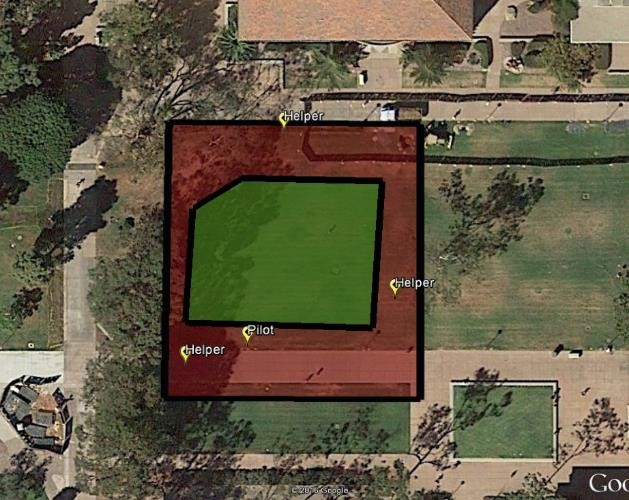
\includegraphics[width=1\linewidth]{images/Mission_Planning_UCSB} 

}

\caption{Mapping out helpers at UCSB}\label{fig:MP-UCSB}
\end{figure}

\hypertarget{on-site-threats}{%
\subsection{On-site Threats}\label{on-site-threats}}

There are many on-site threats to UAS safety that are not always feasible to be reviewed. It is the responsibility of the RPIC to ensure a safe operating environment, from ensuring the unmanned aircraft is suitable for operation to managing intrusions and weather conditions.

\textbf{Example On-site Threats}

\begin{itemize}
\item
  Weather conditions
\item
  Structures not visible from satellite imagery, such as

  \begin{itemize}
  \tightlist
  \item
    Powerlines or telephone poles
  \item
    Recent construction
  \item
    Temporary structures
  \end{itemize}
\item
  Intruding air traffic
\item
  Intruding pedestrians or other non-participants, including wildlife
\item
  unmanned aircraft damage
\item
  Unplanned spectators or crowds
\end{itemize}

\hypertarget{weather}{%
\subsection{Weather}\label{weather}}

Local weather must be checked prior to UAS activity to ensure wind speeds, precipitation, temperature or other environmental factors will not adversely affect the safety of the UAS activity. This information should then be re-checked during the on-site survey, prior to take-off. No UAS activity shall occur when weather conditions exceed VFR Weather minimums or the listed aircraft tolerance per the manufacturer's manual.

\hypertarget{site-permissions}{%
\subsection{Site Permissions}\label{site-permissions}}

All UAS activity at a University Location must have prior authorization, accomplished via the UAS Activity Request Form. If additional authorization is required by a managing entity (campus recreation, Natural Reserve Site Director), it shall be obtained in coordination with the Designated Local Authority or Systemwide Designated UAS Authority. At off-site locations, site permissions shall be obtained as necessary. The UC shall maintain good neighbor relations with all public entities and shall abide by the processes or restrictions as directed.

\textbf{Common Public Land}

\begin{itemize}
\tightlist
\item
  California State Parks - contact the Park Director
\item
  Other California State Agency Land - contact the site director
\item
  National Forest (excluding Wilderness Lands) - No authorization necessary
\end{itemize}

For UAS activity, the RPIC shall obtain site permission to the best of his or her ability for all property the UAS activity will occur above.

\hypertarget{safety-guidelines}{%
\section{Safety Guidelines}\label{safety-guidelines}}

\begin{itemize}
\tightlist
\item
  UAS activity should always establish a buffer or safe-zone between the unmanned aircraft and any non-participating persons or sensitive locations.\\
\item
  A good rule-of-thumb is to maintain a buffer or safe-zone of roughly \(\frac{1}{4}^{th}\) of the flight altitude.\\
\item
  Visual Observers and supporting ground crew should be utilized when available.
\item
  Supporting ground crew should assist in ensuring safety to all non-participating persons.
\item
  High visibility reflective vests should be utilized when operating near roads or when near non-participants (Figure \ref{fig:UASvests}).
\item
  Whistles are effective for alerts or other time-sensitive communication.
\item
  Orange cones may be used to help communicate unmanned aircraft flight regions to non-participating persons, but are not fully sufficient.
\item
  If spectators are expected, a supporting ground crew member should be tasked with preventing spectators from distracting the RPIC with questions or comments.
\item
  When operating in uncontrolled locations in proximity to non-participating persons, extra care should be exercised. Specific flight paths and altitudes should be pre-planned such that potential gaps in buffer or safe-zones can be identified.
\item
  When operating near roads, a supporting ground crew member should be tasked with being located near the road to monitor traffic, and if necessary, retrieve a fallen unmanned aircraft before it becomes a road hazard.
\item
  When operating in fenced areas, operate exclusively within the fenced areas unless there is sufficient visibility on the other side to ensure safety to non-participants.
\item
  Flying above buildings and structures minimizes risk to pedestrians, but it is recommended to contact the facility manager to explain the proposed operation and potential for risk.
\end{itemize}

\begin{figure}

{\centering \includegraphics[width=0.6\linewidth]{images/UAS_Vest} 

}

\caption{UAS Operators with High Visibility Reflective Vests}\label{fig:UASvests}
\end{figure}

\hypertarget{ch-crm}{%
\chapter{Crew Coordination Standards}\label{ch-crm}}

\hypertarget{crew-participant-minimum}{%
\section{Crew Participant Minimum}\label{crew-participant-minimum}}

A member of the Flight Crew must be actively involved in the safety of the UAS activity - this includes participation in pre-flight activities such as planning and briefing, have a well-defined role during the UAS activity and post-flight cleanup. A spectator or spectator crowd may not be `deputized' to a crew member status to circumvent FAA regulations regarding flight operations over people.

\hypertarget{pfb}{%
\section{Pre-Flight Briefing}\label{pfb}}

Briefing is an essential part of conducting UAS activity in a safe and efficient manner. On the day of the flight, prior to the start of UAS activity, the RPIC shall brief all Flight Personnel on the goals, objectives and key safety considerations of the planned UAS activity. The intent is to cover all operation aspects of the UAS activity and to promote full understanding among all Flight Personnel. The guidelines for conducting Flight Personnel briefings are listing below. At a minimum, the RPIC must cover the following in a briefing:

\begin{itemize}
\item
  General Information about the Flight

  \begin{itemize}
  \tightlist
  \item
    Type of Flight (training, maintenance, normal)
  \item
    UAS Status - condition, recent maintenance, fuel or battery state
  \item
    Any mission issues the ground crew should be aware of?
  \end{itemize}
\item
  Crew Members \& their roles and responsibilities. List out by each of the flight phases:

  \begin{itemize}
  \tightlist
  \item
    Before launch
  \item
    During flight
  \item
    In case of an emergency
  \item
    After landing
  \end{itemize}
\item
  Mission Information

  \begin{itemize}
  \tightlist
  \item
    Primary mission goals, any secondary goals
  \item
    Flight Path Detail - estimated duration, flight altitude, flight pattern
  \item
    Landing \& Recovery Procedures
  \end{itemize}
\item
  Site Description and Hazard Analysis

  \begin{itemize}
  \tightlist
  \item
    Hazards and Risks
  \item
    Boundaries
  \item
    Areas of Concern
  \item
    Non-participating Persons
  \item
    Nearby airports or areas of air traffic
  \end{itemize}
\item
  Weather

  \begin{itemize}
  \tightlist
  \item
    Current forecast
  \item
    Weather forecast for the duration of the flight activity
  \item
    Potential weather conditions to monitor
  \end{itemize}
\item
  Communication Procedures

  \begin{itemize}
  \tightlist
  \item
    Chain of command
  \item
    Communication phrasebook
  \end{itemize}
\item
  Mission or Flight Stop/Pause Conditions

  \begin{itemize}
  \tightlist
  \item
    Go/No-Go Conditions (in-flight)
  \item
    Mission Stop Checks (at what conditions should the overall mission be stopped)
  \item
    Flight Stop Checks (at what conditions should an individual flight be stopped)
  \item
    Flight Pause Checks (at what conditions should an individual flight be paused)
  \end{itemize}
\item
  Emergency Management - Roles and Responsibilities during the following situations:

  \begin{itemize}
  \tightlist
  \item
    Non-participating person incursion in flight area
  \item
    Hazardous Weather Conditions
  \item
    Low Battery or UAS Status Issue
  \item
    COllision with Hazard
  \item
    Fly Away or Loss of GPS
  \item
    Lost link or C2 link failure
  \item
    In-Flight or Post-Flight Fire
  \item
    Pilot Incapacitation
  \item
    Manned Aircraft Encroachment in flight area
  \end{itemize}
\item
  Remind the entire crew of the Sterile Cockpit Requirement
\end{itemize}

Public safety should be addressed at every briefing to mitigate all risks from UC flight operations.

\hypertarget{flight-team-member-positioning}{%
\section{Flight Team Member Positioning}\label{flight-team-member-positioning}}

The following factors should be considered when positioning the Flight Team members:

\begin{itemize}
\tightlist
\item
  Visual coverage of the operating site
\item
  Position in relation to the sun to avoid visual impairment
\item
  Physical obstacles such as overhanging trees, rocks, buildings, power lines etc.
\item
  Terrain topography, avoid steep slopes or uneven ground
\item
  Effects such as wind shear from nearby trees, buildings etc
\item
  Proximity to buildings and structures
\end{itemize}

\begin{figure}

{\centering 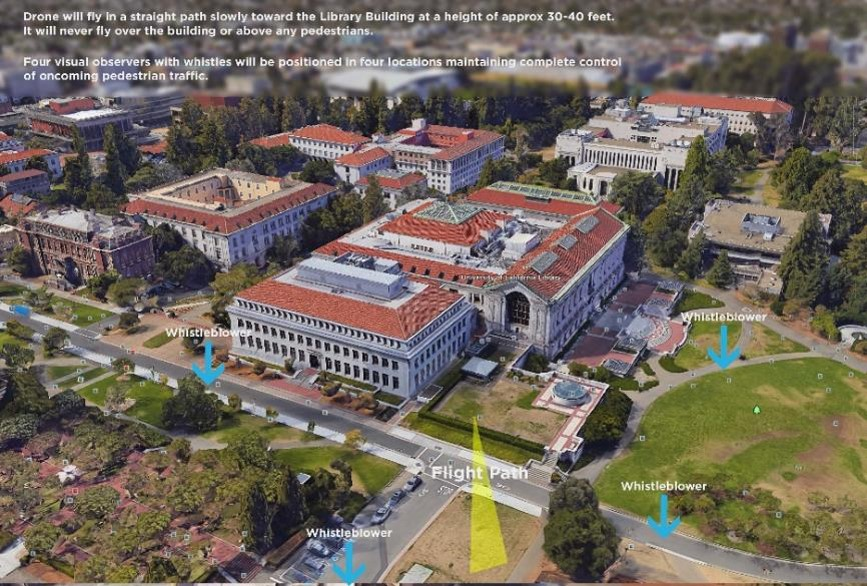
\includegraphics[width=1\linewidth]{images/Mission_Planning_UCB} 

}

\caption{Planning for Safety at UC Berkeley}\label{fig:MP-UCB}
\end{figure}

\hypertarget{sterile-cockpit-requirement}{%
\section{Sterile Cockpit Requirement}\label{sterile-cockpit-requirement}}

After the pre-flight briefing and until the completion of the final cleanup, the RPIC, all Visual Observers and all Ground Support Personnel are prohibited from engaging in non-essential duties or activities.

\textbf{Example failures seen within the UC System:}

\begin{itemize}
\tightlist
\item
  RPIC became distracted while talking with a student and did not recognize that the unmanned aircraft was on a collision course with a floodlight.
\item
  An Ground Support Personnel was engaged in conversation and did not adequately check the unmanned aircraft for loose linkages in between flights, leading to an in-flight failure of the elevator.
\item
  The RPIC was interrupted by a curious bystander.
\item
  Extraneous conversation led to forgetting of the detachable wings of a fixed-wing unmanned aircraft at the lab.
\end{itemize}

\hypertarget{normal-flight-operations}{%
\chapter{Normal Flight Operations}\label{normal-flight-operations}}

\begin{quote}
The Standard Operating Procedures for Advanced UAS Operations (SOPA) applies to the use and guidance of UAS in flight operations, flight planning, training, and oversight as a requirement to exercise the privileges of operating under 1) a Grant of Exemption pursuant to Section 333 of the FAA Modernization and Reform Act of 2012, 2) any Public Agency Operation when operating a Public Aircraft, 3) any other operations conducted under a Certificate of Waiver or Authorization (COA) including an Airspace Authorization, Airspace Waiver or Operational Waiver or 4) any operation categorized as a moderate and above Risk Level. For other Standard Operating Procedures, please see the New User Guide.
\end{quote}

A Normal UAS activity is any flight that is not conducted for training or maintenance purposes.

\begin{itemize}
\tightlist
\item
  Per Policy, all UAS activity requires prior approval granted via the submission of a UAS Activity Request Form.
\item
  It is the responsibility of the RPIC to evaluate each UAS activity in detail prior to operation.
\item
  The Systemwide Designated UAS Authority or Designated Local Authority will evaluate a UAS Activity Request Form for regulatory compliance, identify campus coordination requirements or other requirements necessary to enable UAS activity.
\end{itemize}

\hypertarget{operational-requirements}{%
\section{Operational Requirements}\label{operational-requirements}}

\begin{itemize}
\tightlist
\item
  Before any UAS activity is conducted under the provisions of this SOPA, the RPIC will obtain permission to conduct these operations from all necessary parties. In addition to UC approval, approval may be necessary from property owners and/or local officials as necessary or appropriate. All operations may only be conducted over property where permission has been granted from the owner/ controller or authorized representative.\\
\item
  No UAS activity may occur under the provisions of this SOPA without a completed \protect\hyperlink{ch-mission-binder}{UAS Mission Binder}
\item
  A visual observer is mandatory for all operations under this SOPA.
\end{itemize}

\hypertarget{pre-flight-procedures}{%
\section{Pre-Flight Procedures}\label{pre-flight-procedures}}

\begin{itemize}
\tightlist
\item
  Upon preparing for flight operations, the RPIC is responsible for ensuring that all the necessary information from the completed \protect\hyperlink{ch-mission-binder}{UAS Mission Binder} is available to all flight crew.
\item
  Emergency contact numbers and instructions must be
\item
  Any necessary outstanding mission documentation must be completed prior to flight operations
\item
  All safety equipment, including fire extinguishers must be setup and ready to deploy
\item
  The RPIC must conduct a \protect\hyperlink{pfb}{Pre-Flight Briefing} prior to flight operations
\item
  A Pre-Flight Check is mandatory prior to each flight.
\end{itemize}

\hypertarget{pre-flight-checklist-requirements}{%
\subsection{Pre-Flight Checklist Requirements}\label{pre-flight-checklist-requirements}}

A Pre-Flight Checklist must have, at a minimum, the following checks:

\begin{itemize}
\item
  Inspecting the UAS to ensure it is in a condition for safe flight.

  \begin{itemize}
  \tightlist
  \item
    The UAS must have sufficient fuel or battery capacity to conduct the operation and with a sufficient reserver
  \item
    The Ground Control Station and any other supplemental equipment such as tablets and landing pads, if used, must be included in the Pre-Flight inspection.
  \item
    All payload equipment, including lens and memory cards, is ready for operation
  \end{itemize}
\item
  Evaluating the current conditions of the flight operational area
\item
  Evaluating the current and future weather conditions
\item
  Verifying the flight crew is aware of and capable of conducting their role in a satisfactory manner and are in position.
\item
  Ensuring the airspace and operational area is appropriately clear and safe to operate within
\end{itemize}

\hypertarget{flight-operations}{%
\section{Flight Operations}\label{flight-operations}}

\begin{itemize}
\item
  All Flight Personnel must remain at his or her station as listed in the Flight Operation Plan during takeoff, landing, recovery, and other critical phases of flight, except when performing those duties required for the safe operation of the aircraft.
\item
  The RPIC must ensure that the unmanned aircraft maintains a sufficient power reserve as recommended by the manufacturer.
\item
  The RPIC must terminate the flight and land the unmanned aircraft at any time it appears that the required battery reserves cannot be maintained. When terminating a flight, the primary concern must be the safety of nonparticipating persons.
\item
  All flight operations must be done in accordance to the prepared flight plan and as described during the pre-flight briefing. Intentional deviations are prohibited.

  \begin{itemize}
  \tightlist
  \item
    If a deviation is desired, terminate the flight and prepare a new flight plan.
  \end{itemize}
\end{itemize}

\hypertarget{payload-manipulation}{%
\section{Payload Manipulation}\label{payload-manipulation}}

\begin{itemize}
\tightlist
\item
  If it has been determined that the mission can be safely flown without a separate Payload Operator, the RPIC may not adjust or manipulate the payload in any way unless the aircraft is in a GPS-assisted or autonomous flight mode where there is no danger of collision or loss of control.
\item
  Payload manipulation or adjustment activities must be coordinated with the Visual Observer to ensure adequacy of see-and-avoid procedures and minimum safe distance requirements.
\end{itemize}

\hypertarget{recovery}{%
\section{Recovery}\label{recovery}}

\begin{itemize}
\item
  All UAS landing and recovery will be accomplished in accordance with the Manufacturer's Manual.
\item
  The UAS landing and recovery will take place at the pre-designated landing zone.
\item
  A designated landing zone must be as safe and secure as possible. To the extent possible, the zone should be free of any any obstacles or hazards, including but not limited to:

  \begin{itemize}
  \tightlist
  \item
    Trees or tall brush
  \item
    Fences
  \item
    Large rocks
  \item
    Towers
  \item
    Poles
  \item
    Overhead wires
  \item
    Dust and small pieces of debris
  \item
    Ground vehicles
  \item
    Other aircraft
  \end{itemize}
\item
  Where deemed necessary, Ground Support Personnel will take necessary actions to advise all non-participants to remain a safe distance (typically 10 ft) away laterally away from the landing zone while the unmanned aircraft is landing.
\item
  When possible, locate landing zones such that recovery can be made into the prevailing winds.
\end{itemize}

\hypertarget{shutdownpost-flight}{%
\section{Shutdown/Post-Flight}\label{shutdownpost-flight}}

\begin{itemize}
\item
  UAS shutdown and post flight actions will be taken in accordance with the Manufacturer's Manual.
\item
  The RPIC must complete a post-flight summary using a Post Flight Form. The summary must include, but not be limited to:

  \begin{itemize}
  \tightlist
  \item
    Date
  \item
    Location of Operation (including latitude/longitude)
  \item
    Name(s) and certificate number(s) of the RPIC(s).
  \item
    Registration of the unmanned aircraft to be flown
  \item
    Name of the Point of Contact or Project Manager
  \item
    The names of all flight crew including Visual Observer, Payload Operator or Ground Support Personnel.
  \item
    Duration of Operation
  \item
    Any issues encountered during the operation, including launch or landing damages, lost link, malfunctions, near-misses or other safety issues.
  \end{itemize}
\item
  In the event of an non-emergency safety incident, the RPIC should document the incident and attach all relevant information with the Post Flight Form.\\
\item
  Each lost-link event that occurs during the UAS activity, must be documented in the Post Flight Form.
\item
  The RPIC or a properly trained Visual Observer or Ground Support Personnel must conduct a post flight aircraft inspection as recommended in the Manufacturer's Manual.
\end{itemize}

\hypertarget{emergency-operations}{%
\chapter{Emergency Operations}\label{emergency-operations}}

The recommended procedures for addressing various types of emergencies and critical situations are provided by this Section and in the Manufacturer's Manual. These procedures are suggested as the best practice for coping with the particular conditions described, but are not a substitute for sound judgment and common sense. All personnel, including the RPIC, VO(s) and all Ground Crew engaged in UAS activity under this SOPA should familiarize themselves with the general procedures given in this Section and the Manufacturer's Manual and be prepared to take appropriate action should an emergency arise.

\hypertarget{general-emergency-planning}{%
\section{General Emergency Planning}\label{general-emergency-planning}}

It is required that all UAS activity under this SOPA have a completed emergency procedure plan. A template can be found in \href{https://ucdrones.github.io/ch-resources.html}{UC Drone Resources}.

\textbf{Required Emergency Plans}

\begin{itemize}
\tightlist
\item
  Non-participating person incursion in flight area
\item
  Hazardous Weather Conditions
\item
  Low Battery or UAS Status Issue
\item
  COllision with Hazard
\item
  Fly Away or Loss of GPS
\item
  Lost link or C2 link failure
\item
  In-Flight or Post-Flight Fire
\item
  Pilot Incapacitation
\item
  Manned Aircraft Encroachment in flight area
\end{itemize}

All operations require the RPIC to designate a lost link/emergency termination zones prior to UAS activity. The RPIC retains the right to change or modify that selection if potentially unsafe conditions exist. These zones may be the same location or different locations, depending on the needs of the mission.

The RPIC shall take all necessary actions to ensure that the launch and recover of the unmanned aircraft does not present a hazard to persons and property on the ground. The RPIC, VO and any Ground Crew will take all reasonable actions to ensure all non-essential personnel and nonparticipating persons remain at least 10 feet laterally away from landing zones, including emergency landing zones, while the unmanned aircraft is taking off or landing.

\hypertarget{general-emergency-procedures}{%
\section{General Emergency Procedures}\label{general-emergency-procedures}}

The RPIC is responsible for ensuring flight safety and is responsible for making any assessment in regards to flight safety. If the RPIC is incapacitated for any reason, the responsibility goes to the Visual Observer, unless an alternate has been selected.

In an emergency situation involving the safety of persons or property, which requires immediate decisions and actions, the RPIC or any other appropriate Ground Crew member may take action that is considered necessary under the circumstances to ensure safety.

If, for any reason, the UAS needs to conduct an emergency landing, flight crew personnel, such as the VO or other supporting ground crew will take actions to immediately warn people on the ground below where the unmanned aircraft is operating and alert the RPIC of any potential hazards so that the RPIC can take appropriate action to ensure safe operations of the flight. They must also immediately warn people on the ground below where the unmanned aircraft is operating of any potential hazards associated with the UAS activity.

\begin{quote}
The RPIC may deviate from prescribed operations procedures and methods, weather minimums, regulations, this Manual, etc., to the extent necessary, in the interest of safety.
\end{quote}

A member of the Flight Crew, typically the Visual Observer, shall keep the appropriate ATC facilities fully informed when an in-flight UAS emergency could potentially impact operations of aircraft in navigable air space.

\hypertarget{accident-response}{%
\chapter{Accident Response}\label{accident-response}}

All UAS incidents and accidents must be reported. For minor incidents, this may be done through the normal UAS post-flight reporting system through UC Drones.

For all incidents that result in injury, or property damage of any amount, the Campus Designated Local Authority or the Systemwide Designated UAS Authority must be contacted immediately.

\hypertarget{emergency-contact-information}{%
\section{Emergency Contact Information}\label{emergency-contact-information}}

The emergency contact information for the Systemwide Designated UAS Authority and the Campus Designated Local Authority must be included on the Emergency Procedure Plan and included in the UAS Mission Binder.

\textbf{Systemwide Designated UAS Authority}

\begin{verbatim}
Dr. Brandon Stark
Director, UC Center of Excellence on UAS Safety
(209) 201-2051
UASsafety@ucmerced.edu
\end{verbatim}

\textbf{Designated Local Authority}

See \href{https://ucdrones.github.io/ch-DLA.html}{Campus Points of Contact} for the contact information for each of the UC campuses.

\hypertarget{document-an-accident}{%
\section{Document an accident}\label{document-an-accident}}

As soon as it is safe to,

\begin{itemize}
\item
  Write down a narrative about the incident. Describe what you remember and with as much detail as possible.

  \begin{itemize}
  \tightlist
  \item
    Take note of anything out of the ordinary
  \item
    Include any information that might be relevant for understanding how the incident occured
  \end{itemize}
\item
  Preserve the scene digitally by taking photos and videos
\end{itemize}

\textbf{No one is punished or penalized for reporting an incident or accident. Retribution is not the purpose of documentation. All documentation collected will be used to help improve future practices.}

\hypertarget{fire-safety}{%
\chapter{Fire Safety}\label{fire-safety}}

While UAS accidents and incidents involving fire are rare, they are a valid and significant concern. With the majority of UC UAS usage on field sites and other rural locations, the potential for the accidental sparking of fire is a concern. A fire sparked by a UAS can spread quickly (Figure \ref{fig:fire-start}) and with California's dry environment, can cause significant damage (Figure \ref{fig:fire-damage}).

\begin{figure}

{\centering 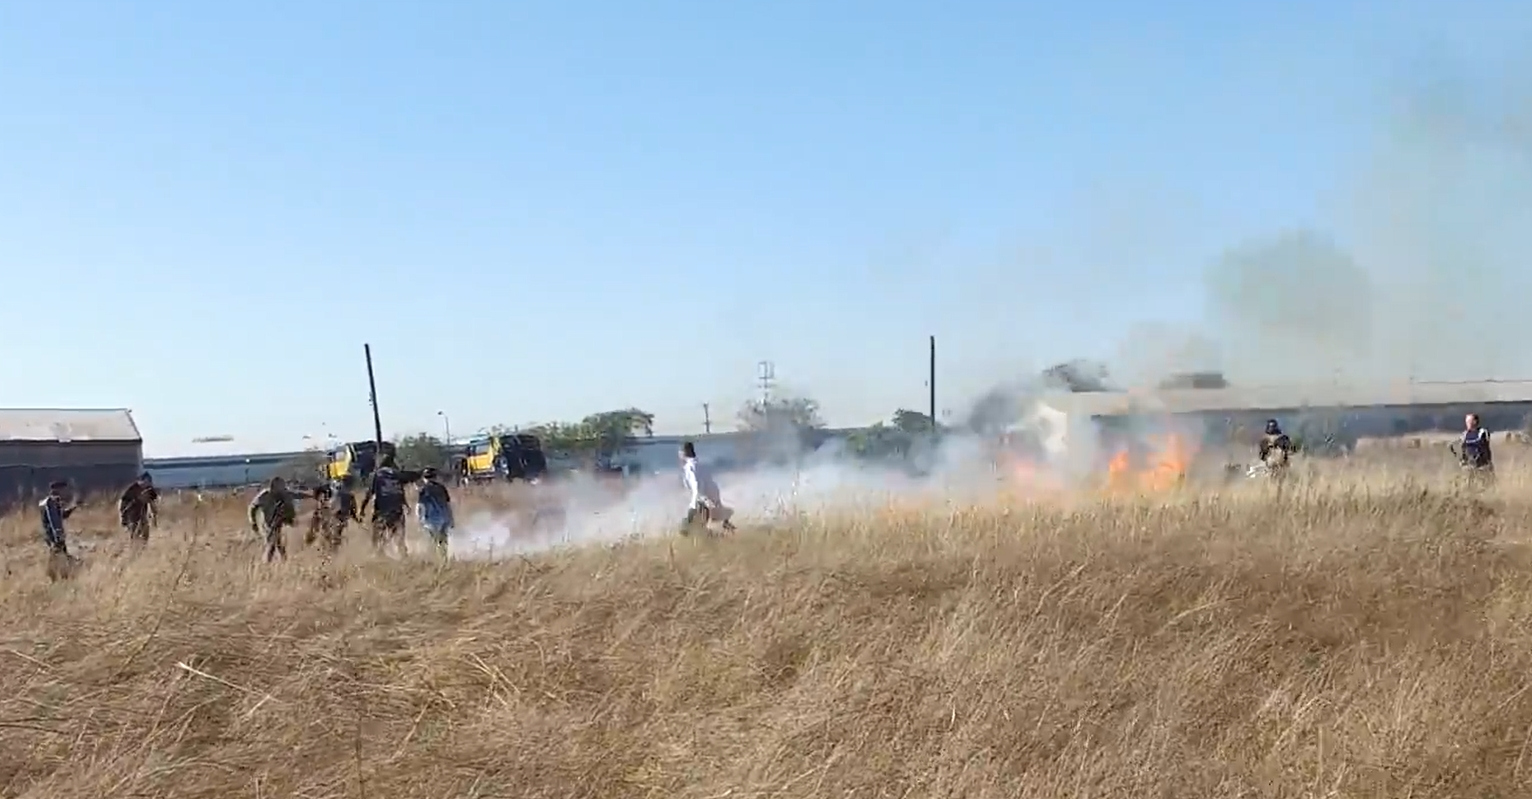
\includegraphics[width=0.75\linewidth]{images/fire_start} 

}

\caption{Beginning of a fire from UAS accident at Richmond Field Station, UC Berkeley}\label{fig:fire-start}
\end{figure}

\begin{figure}

{\centering 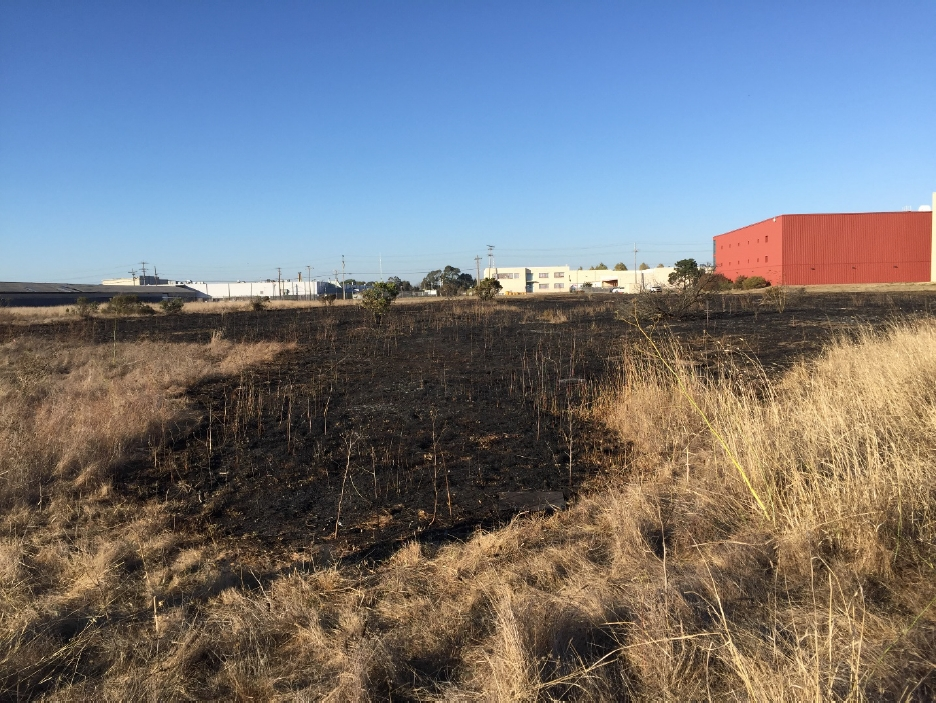
\includegraphics[width=0.75\linewidth]{images/fire_damage} 

}

\caption{Post fire damage from UAS accident at Richmond Field Station, UC Berkeley}\label{fig:fire-damage}
\end{figure}

\hypertarget{lipo-battery-guidance}{%
\section{LiPo Battery Guidance}\label{lipo-battery-guidance}}

The most common cause of UAS related fire is from misuse of LiPo batteries. Special care should be taken when charging, discharging or storing LiPo batteries. If the internal polymer cell of a LiPo battery is exposed to air, a violent chemical reaction starts that could explode, but more commonly releases significant amounts of smoke and heat that can ignite other fire fuel sources. A LiPo battery fire is typically caused by a physical puncture to the battery or from misuse, such as overcharging or electrical shorts.

\textbf{Recommended Best Practices}

\begin{itemize}
\item
  Always thoroughly inspect a battery before charging and use.

  \begin{itemize}
  \tightlist
  \item
    Look for swelling, puffy cells, cracks in plastic, and charred debris along the contacts.
  \end{itemize}
\item
  Never use a battery that is not in good health.

  \begin{itemize}
  \tightlist
  \item
    Consider batteries to be replaceable and consumable, rather than a permanent component of the UAS.
  \end{itemize}
\item
  Never store batteries in a hot car.
\item
  Don't charge your batteries unless you're going to fly within the next day.
\item
  After immediate use, place battery out of the sun but do not place within a closed container.

  \begin{itemize}
  \tightlist
  \item
    Ensure there is sufficient airflow to allow the battery to cool.
  \end{itemize}
\item
  When done flying for the day, always charge your batteries at least back up to storage level.
\item
  Do not charge an intelligent flight battery immediately after flight as the temperature may be too high. Wait until it cools down to room temperature before charging again.
\item
  Store the battery in a dry and cool place, keep out of direct sunlight and away from any liquids
\item
  Do not store or transport a battery with eyeglasses, watches, metal necklaces or other metal components that may short the battery
\item
  When in transport, store the batteries in a safe container that will protect it from damage, squeezing, puncturing or falling.
\end{itemize}

\hypertarget{planning-for-fire-mitigation}{%
\section{Planning for Fire Mitigation}\label{planning-for-fire-mitigation}}

In addition to LiPo battery care, special effort must be taken to consider the fire risks in UAS activity. Consult the appropriate department (Fire, Field Safety, EH\&S) if there are concerns over fire risk. Minimize the potential for fire by monitoring where the UAS will be flying and ensure that if a fire was to occur, the RPIC and any other persons, such as Visual Observers, are prepared to respond appropriately.

\textbf{Guidance for fire safety}

\begin{itemize}
\item
  Everyone should take a fire safety training course.
\item
  Avoid flying on high fire risk days, including \href{https://www.fire.ca.gov/programs/communications/red-flag-warnings-fire-weather-watches/}{Red Flag Warning} alerts issued by CAL FIRE.
\item
  Never fly alone in areas of moderate to high fire risk
\item
  Always bring a fire extinguisher and a shovel/bucket of sand to field sites.
\item
  During flight operations:

  \begin{itemize}
  \tightlist
  \item
    Ensure that a crew member has easy access to fire equipment.
  \item
    Ensure that a crew member has easy access to reach any location where the unmanned aircraft may crash.
  \item
    Ensure that a crew member has the ability to report an emergency situation and can adequately provide directions for emergency personnel to reach the site.
  \end{itemize}
\item
  When flying in high fire risk locations, use high quality, commercially available unmanned aircraft with enclosed electronics.
\item
  Never fly a damaged or swollen battery.
\end{itemize}

\hypertarget{ch-part29waiver}{%
\chapter{Waiver for Operations at Night}\label{ch-part29waiver}}

\hypertarget{s29-gen}{%
\section{General}\label{s29-gen}}

The University of California was granted a Operational Waiver of 14 CFR 107.29 - Daylight Operations (Waiver Number: 107W-2018-1155) for night time UAS activity in Class G airspace.

This Operational Waiver requires modifications to existing UAS activity practices as described in this Standard Operating Procedures for Advanced UAS Operations (SOPA). The following sections document the additional restrictions and addendums to UAS activity necessary to comply with the 14 CFR 107.29 - Daylight Operations Waiver.

\hypertarget{s29-ar}{%
\section{Aircraft Restrictions}\label{s29-ar}}

Unmanned aircraft that operate under this Waiver must meet the following requirements:

\begin{itemize}
\tightlist
\item
  Must be outfitted with an anti-collision strobe light that is visible from a minimum distance of 3 miles.
\item
  Must have navigational lighting that enables the aircraft altitude, attitude and heading to be known through visual observations.
\item
  Must have geofencing capability installed and enabled to prevent unintentional controlled flight outside a safe operating environment
\item
  Must have a real-time data telemetry link that provides the altitude, attitude and heading of the unmanned aircraft
\item
  Must have a real-time data telemetry link that enables an approximate location of the unmanned aircraft at all times, either with GPS coordinates or a flight path overlay on an online map. This information is necessary but not sufficient for navigation purposes.
\end{itemize}

\hypertarget{s29-rr}{%
\section{Addendum to Roles and Responsibilities}\label{s29-rr}}

\textbf{Systemwide Designated UAS Authority}

\begin{itemize}
\item
  The Systemwide Designated UAS Authority is responsible to the FAA for the safe conduct of the operations. Prior to conducting operations that are the

  \begin{itemize}
  \tightlist
  \item
    Must ensure the RPIC, manipulators of the controls, and Visual Observer are informed on the terms and provisions of the Waiver and the strict observance of the terms and provisions herein;
  \item
    Must ensure the RPIC, manipulators of the controls, and Visual Observer are informed and familiar with 14 CFR 107 regulations not waived; and
  \item
    The above must be documented and must be presented for inspection upon request from the Administrator or an authorized representative.
  \end{itemize}
\item
  The Systemwide Designated UAS Authority listed on this Waiver must maintain a current list of pilots by name and remote pilot certificate number used under the Waiver. This list must be presented for inspection upon request from the Administrator or an authorized representative;
\item
  The Systemwide Designated UAS Authority listed on the Waiver must maintain a current list of small unmanned aircraft (sUA) by registration number(s) used under the Waiver. This list must be presented for inspection upon request from the Administrator or an authorized representative;
\end{itemize}

\textbf{Remote Pilot in Command}

\begin{itemize}
\tightlist
\item
  The RPIC must be trained, as described in the Waiver application, to recognize and overcome visual illusions caused by darkness, and understand physiological conditions which may degrade night vision. This training must be documented and must be presented for inspection upon request from the Administrator or an authorized representative.
\end{itemize}

\textbf{Visual Observer}

\begin{itemize}
\tightlist
\item
  One or more Visual Observers is mandatory for all UAS activity under the Waiver.
\item
  The Visual Observer must be trained, as described in the Waiver application, to recognize and overcome visual illusions caused by darkness, and understand physiological conditions which may degrade night vision. This training must be documented and must be presented for inspection upon request from the Administrator or an authorized representative.
\item
  At least one Visual Observer must maintain verbal communication with the RPIC without the need for a radio or electronic devices.
\item
  Auxiliary Visual Observers may utilize a radio or other devices to maintain verbal communication.
\end{itemize}

\hypertarget{s29-fp}{%
\section{Addendum to Flight Planning}\label{s29-fp}}

The following provisions are required for UAS activity under the Waiver

\begin{itemize}
\tightlist
\item
  The area of operation must be sufficiently illuminated to allow both the RPIC and Visual Observer to identify people or obstacles on the ground, or a daytime site assessment must be performed prior to conducting operations that are the subject of this Waiver, noting any hazards or obstructions.
\item
  The unmanned aircraft must be equipped with lighted anti-collision lighting visible from a distance of no less than 3 statute miles. The intensity of the anti-collision lighting may be reduced if, because of operating conditions, it would be in the interest of safety to do so.
\end{itemize}

\hypertarget{s29-wp}{%
\section{Additional Waiver Provisions}\label{s29-wp}}

\begin{itemize}
\tightlist
\item
  The Waiver must not be combined with any other waiver(s), authorizations(s), or exemption(s) without specific authorization from the FAA;
\item
  The FAA has the authority to cancel or delay any or all flight operations if the safety of persons or property on the ground or in the air, are in jeopardy or there is a violation of the terms of the Waiver;
\item
  Operations under the Waiver may only be conducted in Class G airspace unless a separate airspace COA specifically stating that night operations may be conducted in controlled airspace is received from the FAA, in accordance with § 107.41. The airspace COA to operate at night must be requested separately, and is not part of this Waiver;
\item
  A copy of the Waiver must be available during UAS activity that are the subject of the Waiver.
\item
  All operations under the Waiver must use one or more Visual Observer.
\end{itemize}

\hypertarget{s29-tr}{%
\section{Supplementary Training Requirement}\label{s29-tr}}

The UC has developed a supplementary training program that includes an online night flying knowledge course and corresponding knowledge exam. All persons involved in the flight operations must have completed this UAS night flying knowledge course and knowledge exam prior to any operations under the Waiver.

The Online Training can be accessed \href{https://docs.google.com/presentation/d/e/2PACX-1vSfIkWTp24UkUPKk82TTK3Mw_Yp_ScsVnISSmLUjcd-OB7csbv88CxzAgyx6ZbznOSZZCVuDs_g1AIf/pub?start=false\&loop=false\&delayms=3000}{here}. You must pass the quiz at the end with 100\% in order to complete the night flying knowledge course. The completion of the knowledge course is valid only for University of California use - it may not be used for any other purpose.

The knowledge course covers the following material:

\begin{itemize}
\item
  General knowledge of night time operations
\item
  Review of Part 107 requirements
\item
  Equipment

  \begin{itemize}
  \tightlist
  \item
    Anti-Collision lights
  \item
    Navigational Lights\\
  \item
    Situational awareness and environmental equipment
  \end{itemize}
\item
  Operation planning

  \begin{itemize}
  \tightlist
  \item
    Site Inspections
  \item
    Site Evaluations
  \item
    Example Scenarios
  \end{itemize}
\item
  Maintaining visual line of sight at night
\item
  Crew Management for night time operations
\item
  Flight Planning at night
\item
  Visual Illusions and means to combat

  \begin{itemize}
  \tightlist
  \item
    Auto Kinesis
  \item
    False Depth Perception
  \item
    Flicker Vertigo
  \item
    Reversible Perspective Illusion
  \item
    Size and Distance Illusion
  \end{itemize}
\end{itemize}

\hypertarget{s29-wa}{%
\section{Waiver Application}\label{s29-wa}}

\begin{enumerate}
\def\labelenumi{\arabic{enumi}.}
\item
  \textbf{How will the Remote Pilot in Command (Remote PIC) be able to see the aircraft in the dark, at the maximum planned flight distance from the Remote PIC and/or Visual Observer (VO)?}

  Visibility will be ensured through multiple strategies.

  The aircraft will be equipped with a combination of navigational and anti-collision lights. The anti-collision lights (Firehouse Cree Strobe light or equivalent) will be visible for at least 3 miles.

  The operations will only occur during times of clear visibility. This will be determined with a weather report collected no earlier than 12 hours prior to flight activity.

  At least one suitably trained visual observer will be mandatory for all flight operations in the dark and will be strategically located to ensure visibility. The primary visual observer will however be sufficiently close to maintain verbal communication with the RPIC without the need for a radio or phone. Additional auxiliary visual observers may be placed strategically as necessary to establish a safe operation area. Communication by auxiliary VOs may be accomplished through radios or whistles.

  All participants must be in place for at least 30 minutes in the dark to ensure that everyone's eyes have adjusted to the dark.

  \begin{enumerate}
  \def\labelenumii{\arabic{enumii}.}
  \item
    \textbf{How will the remote PIC be able to tell which direction the aircraft is pointing or flying in the dark?}

    Navigational lights (primarily green/red) will enable attitude estimation. Flight activity will remain constrained to within the flight distance both laterally and vertically at which attitude estimation is feasible. The maximum flight distance will be determined through prior validation testing. For systems with limited navigation lights, such as the DJI Mavic Pro, the lateral flight distance will be limited to 50 ft. For systems outfitted with external bright navigation lights (Firehouse Drone UAS Strobe Spot Lights), the maximum distance may be as far as 200-300 ft.
  \item
    \textbf{What procedures will the Remote PIC and/or VO follow in the event that they lose sight of the aircraft in the dark?}

    In the event that the location or attitude estimation of the aircraft cannot be confirmed by either the remote PIC, the flight operation will immediately be paused until visual contact can be restored. If the visual observer loses visual contact, the visual observer will immediately inform the RPIC. If both the visual observer and the RPIC lose visual contact or are unable to determine the attitude of the UAS, the aircraft will be commanded to land immediately using an automated land command.
  \end{enumerate}
\item
  \textbf{How will the Remote PIC and/or VO locate other persons, aircraft, obstacles, and structures in the dark?}

  No earlier than 12 hours prior to flight operations, all RPICs and VOs will be required to conduct both a daylight site inspection and site evaluation. The site inspection will consist of identifying potential obstacles, structures and points of access for non-participating persons or vehicles. The evaluation will consist of evaluating mitigation strategies for obstacle avoidance and establishing means to ensure the site will remain clear of non-participating persons. Mitigation strategies for obstacle avoidance include establishing appropriate operating limits and means for identifying the limits of the operations in the dark. Means to ensure the site will remain clear of non-participating persons include evaluating and procuring if necessary, pedestrian traffic control such as reflective traffic cones and reflective caution tape. Auxiliary VOs may be placed at strategic points to assist in preventing non-participating pedestrian or vehicular traffic.

  For the detection and threat evaluation of other aircraft, the RPIC and VOs training will include how to listen for aircraft and conduct a threat evaluation including a follow-up visual search for intruding aircraft.

  \begin{enumerate}
  \def\labelenumii{\arabic{enumii}.}
  \item
    \textbf{What will they do if other persons/aircraft are located during flight?}

    In the event of a breach of the operation site by non-participant or the detection of an aircraft within the vicinity, the flight operation will be immediately paused and a threat assessment will be conducted. Pausing the mission will consist of hovering and keeping the drone in place. To do a threat assessment, the RPIC and the VOs will discuss the situation and evaluate contingency operations. Determining the best course of action will depend on the threat assessment, some possible courses of action include but are not limited to: Hovering in place until the threat is resolved, landing immediately or even moving our landing area to another space. In the event of an imminent threat to safety, the RPIC will take emergency actions without consultation with the VOs.
  \item
    \textbf{How will they avoid hitting obstacles/structures during flight?}

    No earlier than 12 hours prior to flight operations, all RPICs and VOs will be required to conduct both a site inspection and evaluation. The site inspection will consist of identifying potential obstacles, structures and points of access for non-participating persons or vehicles. The evaluation will consist of evaluating mitigation strategies for obstacle avoidance and establishing means to ensure the site will remain clear of non-participating persons. Mitigation strategies for obstacle avoidance include establishing appropriate operating limits and means for identifying the limits of the operations in the dark. Means to ensure the site will remain clear of non-participating persons include evaluating and procuring if necessary, pedestrian traffic control such as reflective traffic cones and reflective caution tape. During the flight operation, the VO(s) will be tasked to monitor the aircraft for proximity to obstacles and structures.
  \item
    \textbf{If flight operations occur in an area with lighting sufficient for the Remote PIC and VO to see their aircraft, and other obstacles, persons, and aircraft, how will they determine the lighting is sufficient prior to flight?}

    The lighting system for the aircraft consists of navigational lights and anti-collision lights. If the light operations occur in an area with lighting sufficient for the Remote PIC and VO to see the aircraft (normally met by navigation lights) and other obstacles (normally met through mitigation strategies), there remains the issue of determining whether the lighting system is sufficient for anti-collision purposes. The aircraft will be outfitted with an anti-collision strobe light that is visible from a minimum distance of 3 miles. Given that the ambient lighting may attenuate the maximum visibility distance of the strobe light, the strobe light must be evaluated in a similar lighting condition.
  \end{enumerate}
\item
  \textbf{While keeping eyes on the aircraft, how will the Remote PIC continuously know their aircraft's current real-time (1) geographic location, (2) altitude above the ground, (3) attitude (orientation, deck angle, pitch, bank) and (4) direction of flight?}

  The aircrafts used within this waiver must have a real-time data telemetry link that provides the (2) altitude above the ground, (3) attitude and (4) direction of flight. The real-time data telemetry link must also provide GPS coordinates and an option to overlay the aircraft position on an online map. It is recognized that the online map may not be up-to-date and thus may be unreliable for accurate (1) geographic location. As such, prior to flight, a site inspection and evaluation must be made, and a visual observer may be tasked with providing accurate (1) geographic location information verbally to the RPIC.
\item
  \textbf{How will the Remote PIC and any other persons participating in the operation demonstrate knowledge about night operation risks, such as overcoming night visual illusions, limitations to night vision and conditions that can affect night vision?}

  All persons involved in the flight operations must have completed a UAS night flying knowledge course and must annually pass a knowledge exam with an \(100\%\) passing score. The knowledge course will include issues such as overcoming night visual illusions and other mitigation strategies for air safety.

  \begin{enumerate}
  \def\labelenumii{\arabic{enumii}.}
  \item
    \textbf{How will this knowledge be obtained and who will document it?}

    All persons involved in the flight operations must have completed a UAS night flying knowledge course and must annually pass a knowledge exam. If a crew member receives less than \(100\%\), the crew member must have the exam reviewed and corrected until he or she reaches \(100\%\). A certificate of completion of the course and the exam with a passing score must be submitted to the Responsible Person and through the University of California UAS Safety Management System.
  \item
    \textbf{How will the responsible person verify that it has been obtained and documented?}

    The University of California employs a UAS Safety Management System and coordinates all official UAS activity through a centralized office.

    The coordination system includes a detailed listing of UC approved UAS pilots and aircraft, mandatory pre-flight assessments and mandatory flight reporting for each flight in order to continuously improve UAS safety and reliability, while providing accountability for all UAS activity. The coordination enables the responsible person to validate whether the RPIC and any ground crew has taken the knowledge course and knowledge exam.

    The list of UC approved pilots and aircraft, as well as any applicable flight records, will be made available to the FAA upon request.
  \end{enumerate}
\item
  \textbf{How Will the aircraft be visible for at least 3 statute miles (SM) at night, in the location you will operate at?}

  The aircraft must have an anti-collision strobe light installed (Firehouse Cree Strobe light or equivalent) that is visible to at least 3 statute miles. The visibility distance must be validated prior to use in operations where ambient light may attenuate the maximum visibility.
\end{enumerate}

\hypertarget{ch-part39-vantage}{%
\chapter{Waiver for Operations over People - Vantage Robotics SNAP}\label{ch-part39-vantage}}

\hypertarget{s39v-gen}{%
\section{General}\label{s39v-gen}}

UAS activity over people (other than Flight Personnel) are prohibited under 14 CFR 107 unless the operator has been granted an FAA Certificate of Waiver that waives the prohibition in 14 CFR 107.39 on flights over human beings that are not directly participating in the operation of the UAS or located under a covered structure or inside a stationary vehicle that can provide reasonable protection from a falling unmanned aircraft.

The University of California was granted an Operational Waiver of 14 CFR 107.39(a) - Operation over Human Beings (Waiver Number: 107W-2019-00336). This waiver is specific for the Vantage Robotics Snap, in Class G airspace, and only in accordance with the provisions within this manual. The following is an addendum to the previous operational instructions within this manual.

\hypertarget{s39v-ar}{%
\section{Aircraft Restrictions}\label{s39v-ar}}

\begin{itemize}
\tightlist
\item
  Operations conducted under this Waiver may only occur with the Vantage Robotics Snap. Proposed operations of any other unmanned aircraft will require a new waiver application or an application to amend the Waiver;
\item
  Any UAS that has undergone maintenance that affects the UAS operation or flight characteristics (e.g., replacement of a flight critical component), must undergo a functional test flight prior to conducting operations under this Waiver. The functional test flight may only be conducted in accordance with requirements of part 107 (without waiver). Operations over human beings during functional test flights are prohibited;
\item
  Any modification to the UAS design is prohibited. Repair and replacement of damaged components is allowed, provided the replacement part is exactly the same as the original. No substitutions are allowed unless a new waiver application is submitted;
\end{itemize}

\hypertarget{s39v-rr}{%
\section{Addendum to Roles and Responsibilities}\label{s39v-rr}}

The following items are added to the respective Roles and Responsibilities.

\textbf{System Designated UAS Authority}

\begin{itemize}
\item
  The Systemwide Designated UAS Authority listed on the Operational Waiver is responsible for the safe conduct of operations. Prior to conducting UAS activity that are subject of the waiver, the Systemwide Designated UAS Authority :

  \begin{itemize}
  \tightlist
  \item
    Must ensure all Direct Participants are informed of the terms and provisions of this Waiver and the strict observance of the terms and provisions herein,
  \item
    Must ensure all Direct Participants are informed and familiar with part 107 regulations not waived, and
  \item
    The Systemwide Designated UAS Authority must keep a record of the communications that establish compliance with the above paragraphs. This record must be presented for inspection upon request by the Administrator or an authorized representative;
  \end{itemize}
\item
  The Systemwide Designated UAS Authority listed on this Waiver must maintain a current list of unmanned aircraft by registration number(s) used in the UAS activity that are subject to the waiver. The Vantage Robotics Snap is the only type of UAS approved for use for operations conducted in accordance with this waiver. This list must be presented for inspection upon request by the Administrator or an authorized representative;
\item
  The Systemwide Designated UAS Authority listed on this Waiver must maintain a current list of remote pilots by name and remote pilot certificate number used in the UAS activity that are subject to the waiver. This list must be presented for inspection upon request by the Administrator or an authorized representative;
\item
  The Systemwide Designated UAS Authority must maintain the sUAS and its components in accordance with manufacturer's instructions. The aircraft manufacturer may provide the maintenance program, or, if one is not provided, the Responsible Person must develop one prior to performing sUAS operations that are the subject of this waiver. sUAS maintenance includes scheduled and unscheduled overhaul, repair, inspection, modification, replacement, and system software upgrades of the sUAS and its components that are necessary for flight. Each sUAS operated under this Waiver must comply with all manufacturer safety bulletins. Records of this maintenance must be retained for 90 days after the expiration date of the waiver;
\item
  If the intended operation would be contrary to or obviate a common or special provision of this waiver, then the Systemwide Designated UAS Authority must apply for an amendment to this Waiver;
\item
  If a discrepancy exists between the special provisions in this Waiver and the procedures outlined in the waiver application, the provisions herein take precedence and must be followed. Otherwise, the Systemwide Designated UAS Authority must follow all procedures as described in the waiver application;
\end{itemize}

\textbf{Remote Pilot in Command}

\begin{itemize}
\tightlist
\item
  An RPIC operating under this waiver must have at least 5 hours of flight training with the UAS
\item
  The RPIC must have conducted at least 3 launch and recovery operations within the last 6 months with the UAS to be considered current.
\item
  The RPIC must have completed a UAS Operations Over People knowledge course and must annually pass a knowledge exam with a passing score of 100\(\%\). A certificate of completion of the course and the exam with a passing score must be submitted to the Designated Local Authority and the Systemwide Designated UAS Authority, and must be available while on-site.
\end{itemize}

\textbf{Visual Observer}

\begin{itemize}
\tightlist
\item
  At least two Visual Observers are required for any operation under this waiver.
\item
  No one may operate as a Visual Observer unless they have read and familiarized themselves with the content of the Part 39 waiver.
\item
  The Visual Observer must have completed a UAS Operations Over People knowledge course and must annually pass a knowledge exam with a passing score of 100\(\%\). A certificate of completion of the course and the exam with a passing score must be submitted to the Designated Local Authority and the Systemwide Designated UAS Authority, and must be available while on-site.
\item
  At least one Visual Observer must maintain verbal communication with the RPIC without the need for a radio or electronic devices.
\item
  Auxiliary Visual Observers may utilize a radio or other devices to maintain verbal communication.
\item
  At least one Visual Observer must be sufficiently trained to land the unmanned aircraft in the event that the RPIC is incapacitated, and must be able to take command of the unmanned aircraft within 10 seconds.
\end{itemize}

\hypertarget{s39v-fp}{%
\section{Addendum to Flight Planning}\label{s39v-fp}}

The following provisions are required for UAS activity under the Waiver:

\begin{itemize}
\tightlist
\item
  The FAA has the authority to cancel or delay any or all flight operations in order to maintain safety or to ensure compliance with the terms of this Waiver;
\item
  This Waiver must not be combined with any other waiver(s), authorizations(s), or exemption(s) without specific, prior authorization;
\item
  Operations under this Waiver are to be conducted in Class G airspace only unless specific airspace authorization or waiver is received from the FAA in accordance with § 107.41;
\item
  A copy of this Waiver must be available during the sUAS operations that are the subject of this Waiver;
\item
  Operations over all human beings (including Nonparticipants) are permitted;
\item
  The sUA must not be operated higher than 150 feet above ground level (AGL) when operated over Nonparticipants in accordance with this Waiver. Any altitude restriction lower than 150 AGL specified in an airspace authorization the FAA grants for operations conducted in accordance with this Waiver takes precedence;
\item
  Flight Personnel must be easily identifiable visually (e.g.~apparel, safety vests);
\item
  The location and time of UAS activity must be selected to provide the maximum safety of people and equipment, and UAS activity must be conducted only if necessary. The decision to operate above people is not to be considered lightly and other options must be considered first.
\end{itemize}

\hypertarget{s39v-rk}{%
\section{Record Keeping Requirements}\label{s39v-rk}}

Records shall be maintained for each flight conducted under the terms of this waiver, and records must be retained for a period of 90 days after the expiration date of the Waiver. The Responsible Person shall keep these records at its principal place of business or at other places approved by the Administrator, and shall make the records available for inspection by request of the Administrator. Each record should contain the following:

\begin{itemize}
\item
  Date, Name of Operator, Responsible Person, Waiver number and Aircraft registration number
\item
  All operating locations, to include location city/name and latitude/longitude
\item
  Number of flights (per location, per aircraft)
\item
  Total aircraft operational hours
\item
  Approximate average altitude of flight
\item
  Equipment malfunctions. Reportable malfunctions include, but are not limited to the following:

  \begin{itemize}
  \tightlist
  \item
    On-board flight control system
  \item
    Navigation system
  \item
    Power plant failure in flight
  \item
    Electrical system failure
  \item
    Control station failure
  \item
    Any failure or malfunction that was followed by a ground collision
  \end{itemize}
\item
  The number and duration of lost link events per sUA per flight.
\item
  Number of people, if any, impacted by the sUA
\item
  Descriptions of any injuries that anyone suffers as a result of an impact with the sUA.
\end{itemize}

\hypertarget{s39v-tr}{%
\section{Supplementary Training Requirement}\label{s39v-tr}}

The UC has developed a supplementary training program that includes an online Operations over People knowledge course and corresponding knowledge exam. All persons involved in the flight operations must have completed this UAS Operations over People knowledge course and knowledge exam prior to any operations under the Waiver.

The knowledge course covers the following material:

\begin{itemize}
\item
  General knowledge of Operations over People
\item
  Review of Part 107 requirements

  \begin{itemize}
  \tightlist
  \item
    Aeronautical Decision Making
  \item
    Crew Resource Management
  \end{itemize}
\item
  Equipment

  \begin{itemize}
  \tightlist
  \item
    Vantage Robotics Snap
  \item
    Operation Modes
  \item
    Failsafe Features
  \end{itemize}
\item
  Operation planning

  \begin{itemize}
  \item
    Site Inspections
  \item
    Site Evaluations
  \item
    Example Scenarios

    \begin{itemize}
    \tightlist
    \item
      Closed-set filming
    \item
      Sparse Crowds at Events
    \end{itemize}
  \end{itemize}
\item
  Emergency Management

  \begin{itemize}
  \item
    Air Traffic Avoidance Procedures
  \item
    Optical Illusions

    \begin{itemize}
    \tightlist
    \item
      Auto Kinesis
    \item
      False Depth Perception
    \item
      Flicker Vertigo
    \item
      Reversible Perspective Illusion
    \item
      Size and Distance Illusion
    \end{itemize}
  \end{itemize}
\end{itemize}

\hypertarget{ch-part39-parazero}{%
\chapter{Waiver for Operations over People - ParaZero}\label{ch-part39-parazero}}

\hypertarget{s39p-gen}{%
\section{General}\label{s39p-gen}}

UAS activity over people (other than Flight Personnel) are prohibited under 14 CFR 107 unless the operator has been granted an FAA Certificate of Waiver that waives the prohibition in 14 CFR 107.39 on flights over human beings that are not directly participating in the operation of the UAS or located under a covered structure or inside a stationary vehicle that can provide reasonable protection from a falling unmanned aircraft.

The University of California was granted an Operational Waiver of 14 CFR 107.39(a) - Operation over Human Beings (Waiver Number: 107W-2019-04492). This waiver is specific for DJI Mavic 2 series UAS with the ParaZero SaveAir Mavic and ASTM Professional Kit installed. This waiver is only applicable within Class G airspace, and may only be utilized in accordance with the provisions within this manual. The following is an addendum to the previous operational instructions within this manual.

\hypertarget{s39p-ar}{%
\section{Aircraft Restrictions}\label{s39p-ar}}

\begin{itemize}
\tightlist
\item
  Operations conducted under this Waiver may only occur with DJI Mavic 2 series UAS equipped with the ParaZero SafeAir parachute system and in compliance with ASTM F3322-18 Standard Specifications for sUAS parachutes.
\item
  The parachute must be packed or repacked by the manufacturer or a manufacturer certified repacker. If the SafeAir system has been opened or deployed, contact \href{mailto:support@parazero.com}{\nolinkurl{support@parazero.com}} to receive shipping instructions for repacking.
\item
  Any UAS that has undergone maintenance that affects the UAS operation or flight characteristics (e.g., replacement of a flight critical component), must undergo a functional test flight prior to conducting operations under this Waiver. The functional test flight may only be conducted in accordance with requirements of part 107 (without waiver). Operations over human beings during functional test flights are prohibited;
\item
  Any modification to the UAS design is prohibited. Repair and replacement of damaged components is allowed, provided the replacement part is exactly the same as the original. No substitutions are allowed unless a new waiver application is submitted;
\end{itemize}

\hypertarget{s39p-rr}{%
\section{Addendum to Roles and Responsibilities}\label{s39p-rr}}

The following items are added to the respective Roles and Responsibilities.

\textbf{System Designated UAS Authority}

\begin{itemize}
\item
  The Systemwide Designated UAS Authority listed on the Operational Waiver is responsible for the safe conduct of operations. Prior to conducting UAS activity that are subject of the waiver, the Systemwide Designated UAS Authority :

  \begin{itemize}
  \tightlist
  \item
    Must ensure all Direct Participants are informed of the terms and provisions of this Waiver and the strict observance of the terms and provisions herein,
  \item
    Must ensure all Direct Participants are informed and familiar with part 107 regulations not waived, and
  \item
    The Systemwide Designated UAS Authority must keep a record of the communications that establish compliance with the above paragraphs. This record must be presented for inspection upon request by the Administrator or an authorized representative;
  \end{itemize}
\item
  The Systemwide Designated UAS Authority listed on this Waiver must maintain a current list of unmanned aircraft by registration number(s) and SafeAir parachute system serial number used in the UAS activity that are subject to the waiver. This list must be presented for inspection upon request by the Administrator or an authorized representative;
\item
  The Systemwide Designated UAS Authority listed on this Waiver must maintain a current list of remote pilots by name and remote pilot certificate number used in the UAS activity that are subject to the waiver. This list must be presented for inspection upon request by the Administrator or an authorized representative;
\item
  The Systemwide Designated UAS Authority must maintain the sUAS and its components in accordance with manufacturer's instructions. The aircraft manufacturer may provide the maintenance program, or, if one is not provided, the Responsible Person must develop one prior to performing sUAS operations that are the subject of this waiver. sUAS maintenance includes scheduled and unscheduled overhaul, repair, inspection, modification, replacement, and system software upgrades of the sUAS and its components that are necessary for flight. Each sUAS operated under this Waiver must comply with all manufacturer safety bulletins. Records of this maintenance must be retained for 90 days after the expiration date of the waiver;
\item
  If the intended operation would be contrary to or obviate a common or special provision of this waiver, then the Systemwide Designated UAS Authority must apply for an amendment to this Waiver;
\item
  If a discrepancy exists between the special provisions in this Waiver and the procedures outlined in the waiver application, the provisions herein take precedence and must be followed. Otherwise, the Systemwide Designated UAS Authority must follow all procedures as described in the waiver application;
\end{itemize}

\textbf{Remote Pilot in Command}

\begin{itemize}
\tightlist
\item
  An RPIC operating under this waiver must have at least 5 hours of flight training with the UAS
\item
  The RPIC must have conducted at least 3 launch and recovery operations within the last 6 months with the UAS to be considered current.
\item
  The RPIC must have completed a UAS Operations Over People knowledge course and must annually pass a knowledge exam with a passing score of 100\(\%\). A certificate of completion of the course and the exam with a passing score must be submitted to the Designated Local Authority and the Systemwide Designated UAS Authority, and must be available while on-site.
\item
  The ASTM documentation provided by ParaZero must be submitted to the Systemwide Designated UAS Authority before use.
\end{itemize}

\textbf{Visual Observer}

\begin{itemize}
\tightlist
\item
  At least two Visual Observers are required for any operation under this waiver.
\item
  No one may operate as a Visual Observer unless they have read and familiarized themselves with the content of the Part 39 waiver.
\item
  The Visual Observer must have completed a UAS Operations Over People knowledge course and must annually pass a knowledge exam with a passing score of 100\(\%\). A certificate of completion of the course and the exam with a passing score must be submitted to the Designated Local Authority and the Systemwide Designated UAS Authority, and must be available while on-site.
\item
  At least one Visual Observer must maintain verbal communication with the RPIC without the need for a radio or electronic devices.
\item
  Auxiliary Visual Observers may utilize a radio or other devices to maintain verbal communication.
\item
  At least one Visual Observer must be sufficiently trained to land the unmanned aircraft in the event that the RPIC is incapacitated, and must be able to take command of the unmanned aircraft within 10 seconds.
\end{itemize}

\hypertarget{s39p-fp}{%
\section{Addendum to Flight Planning}\label{s39p-fp}}

The following provisions are required for UAS activity under the Waiver:

\begin{itemize}
\tightlist
\item
  The FAA has the authority to cancel or delay any or all flight operations in order to maintain safety or to ensure compliance with the terms of this Waiver.
\item
  This Waiver must not be combined with any other waiver(s), authorizations(s), or exemption(s) without specific, prior authorization.
\item
  Operations under this Waiver are to be conducted in Class G airspace only unless specific airspace authorization or waiver is received from the FAA in accordance with § 107.41.
\item
  A copy of this Waiver must be available during the sUAS operations that are the subject of this Waiver.
\item
  Operations over all human beings (including nonparticipants) are permitted.
\item
  Operations may not occur over moving vehicles.
\item
  The sUA must be flown at a minimum at least 70 ft AGL when above nonparticipants.
\item
  Flight Personnel must be easily identifiable visually (e.g.~apparel, safety vests).
\item
  The location and time of UAS activity must be selected to provide the maximum safety of people and equipment, and UAS activity must be conducted only if necessary. The decision to operate above people is not to be considered lightly and other options must be considered first.
\item
  If the UAS loses communications or loses its GPS signal, the UAS must return to a predetermined location within the operating area and land. The PIC must abort the flight in the event of unpredicted obstacles or emergencies. If all standard reconnection procedures fail, the RPIC has the ability to safely terminate the flight by manually triggering the SafeAir System if the sUAS does drift towards an area that is deemed to be higher risk.
\end{itemize}

\hypertarget{s39p-rk}{%
\section{Record Keeping Requirements}\label{s39p-rk}}

Records shall be maintained for each flight conducted under the terms of this waiver, and records must be retained for a period of 90 days after the expiration date of the Waiver. The Responsible Person shall keep these records at its principal place of business or at other places approved by the Administrator, and shall make the records available for inspection by request of the Administrator. Each record should contain the following:

\begin{itemize}
\item
  Date, Name of Operator, Responsible Person, Waiver number and Aircraft registration number
\item
  All operating locations, to include location city/name and latitude/longitude
\item
  Number of flights (per location, per aircraft)
\item
  Total aircraft operational hours
\item
  Approximate average altitude of flight
\item
  Equipment malfunctions. Reportable malfunctions include, but are not limited to the following:

  \begin{itemize}
  \tightlist
  \item
    On-board flight control system
  \item
    Navigation system
  \item
    Power plant failure in flight
  \item
    Electrical system failure
  \item
    Control station failure
  \item
    Any failure or malfunction that was followed by a ground collision
  \end{itemize}
\item
  The number and duration of lost link events per sUA per flight.
\item
  Number of people, if any, impacted by the sUA
\item
  Descriptions of any injuries that anyone suffers as a result of an impact with the sUA.
\end{itemize}

\hypertarget{s39p-tr}{%
\section{Supplementary Training Requirement}\label{s39p-tr}}

The UC has developed a supplementary training program that includes an online Operations over People knowledge course and corresponding knowledge exam. All persons involved in the flight operations must have completed this UAS Operations over People knowledge course and knowledge exam prior to any operations under the Waiver.

The knowledge course covers the following material:

\begin{itemize}
\item
  General knowledge of Operations over People
\item
  Review of Part 107 requirements

  \begin{itemize}
  \tightlist
  \item
    Aeronautical Decision Making
  \item
    Crew Resource Management
  \end{itemize}
\item
  Equipment

  \begin{itemize}
  \tightlist
  \item
    DJI Mavic 2 series
  \item
    ParaZero SafeAir parachute system setup
  \item
    ParaZero ASTM compliance
  \end{itemize}
\item
  Operation planning

  \begin{itemize}
  \item
    Site Inspections
  \item
    Site Evaluations
  \item
    Example Scenarios

    \begin{itemize}
    \tightlist
    \item
      Closed-set filming
    \item
      Sparse Crowds at Events
    \end{itemize}
  \end{itemize}
\item
  Emergency Management

  \begin{itemize}
  \item
    Air Traffic Avoidance Procedures
  \item
    Optical Illusions

    \begin{itemize}
    \tightlist
    \item
      Auto Kinesis
    \item
      False Depth Perception
    \item
      Flicker Vertigo
    \item
      Reversible Perspective Illusion
    \item
      Size and Distance Illusion
    \end{itemize}
  \end{itemize}
\end{itemize}

\end{document}
